\newpage
\textbf{\huge Chapter 3}
\section{METHODOLOGY}
\begin{justify}
This chapter describes the complete pipeline from raw reviews to business intelligence output. Figure~\ref{fig:pipeline} gives an overview of the system architecture.
\end{justify}

\begin{figure}[H]
    \centering
    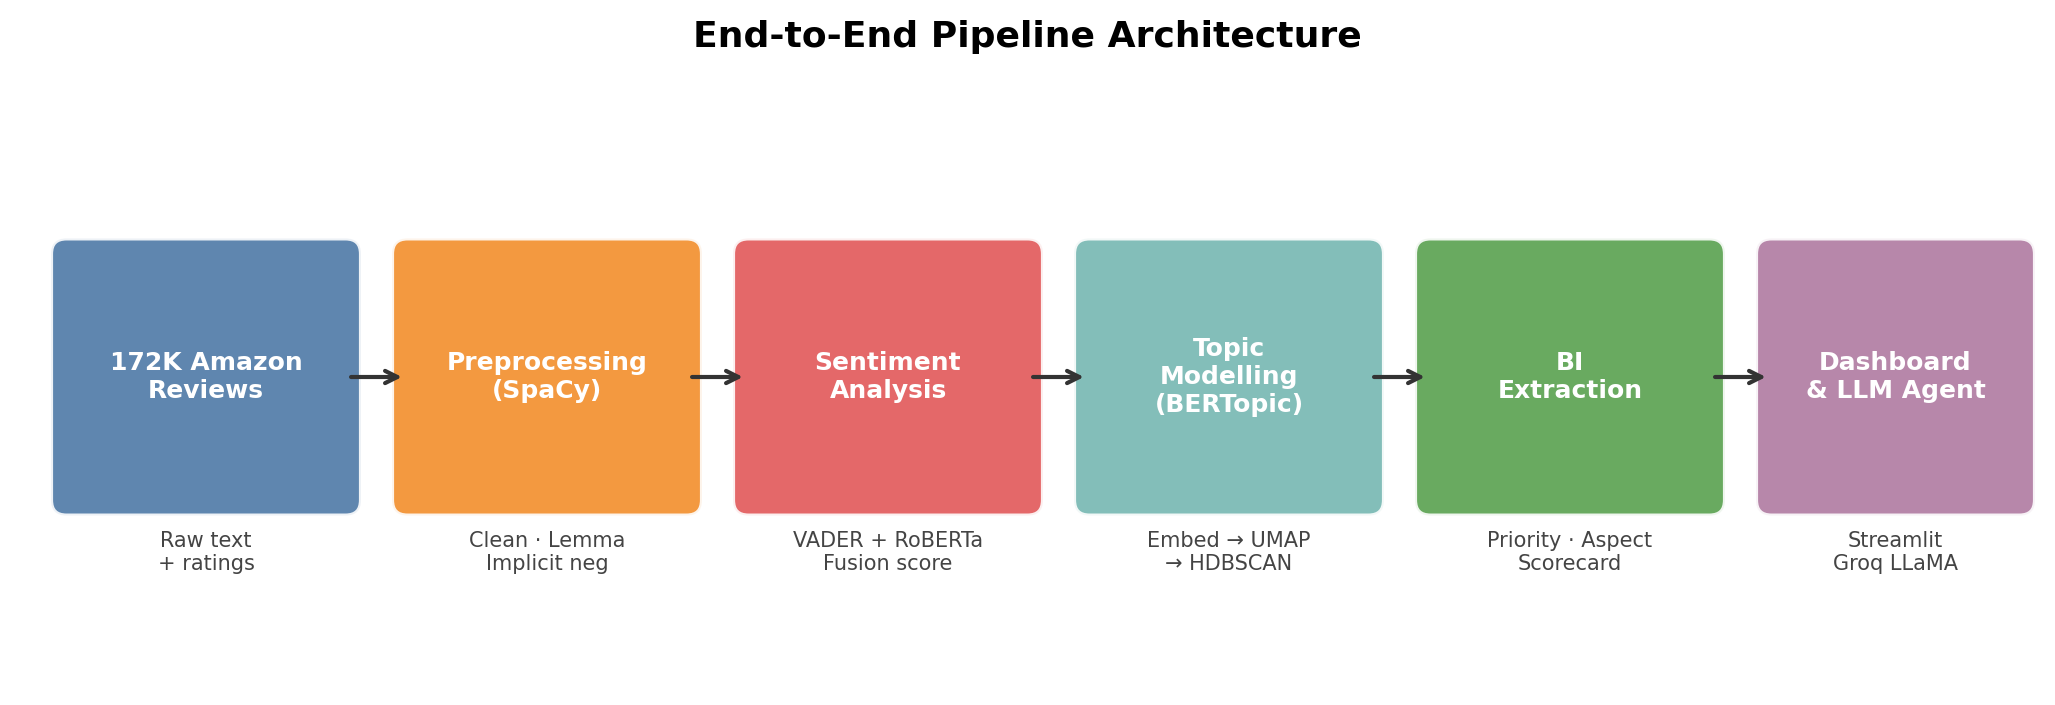
\includegraphics[width=\linewidth]{images/pipeline.png}
    \caption{System architecture: end-to-end pipeline from raw reviews to business intelligence dashboard.}
    \label{fig:pipeline}
\end{figure}

\subsection{Dataset}
\begin{justify}
The dataset used in this project contains \textbf{172,718 Amazon product reviews} spread across six product categories, selected to ensure balanced representation for cross-category comparison. Each record includes the review text, star rating (1--5), product category, reviewer ID, and timestamp.

\begin{table}[H]
\centering
\caption{Dataset Statistics by Category}
\renewcommand{\arraystretch}{1.3}
\begin{tabular}{|l|r|r|r|r|}
\hline
\textbf{Category} & \textbf{Reviews} & \textbf{Avg. Rating} & \textbf{Avg. Tokens} & \textbf{\% 3-Star} \\
\hline
Electronics                  & $\sim$28,786 & 3.9 & 82 & 11.2\% \\
Home and Kitchen             & $\sim$28,786 & 4.1 & 74 & 10.8\% \\
Clothing Shoes and Jewelry   & $\sim$28,786 & 4.0 & 68 & 11.5\% \\
Sports and Outdoors          & $\sim$28,786 & 4.2 & 71 & 10.1\% \\
Grocery and Gourmet Food     & $\sim$28,786 & 4.3 & 65 & 9.7\%  \\
Toys and Games               & $\sim$28,786 & 4.1 & 77 & 11.3\% \\
\hline
\textbf{Total}               & \textbf{172,718} & \textbf{4.1} & \textbf{73} & \textbf{10.8\%} \\
\hline
\end{tabular}
\label{tab:dataset}
\end{table}

\begin{figure}[H]
    \centering
    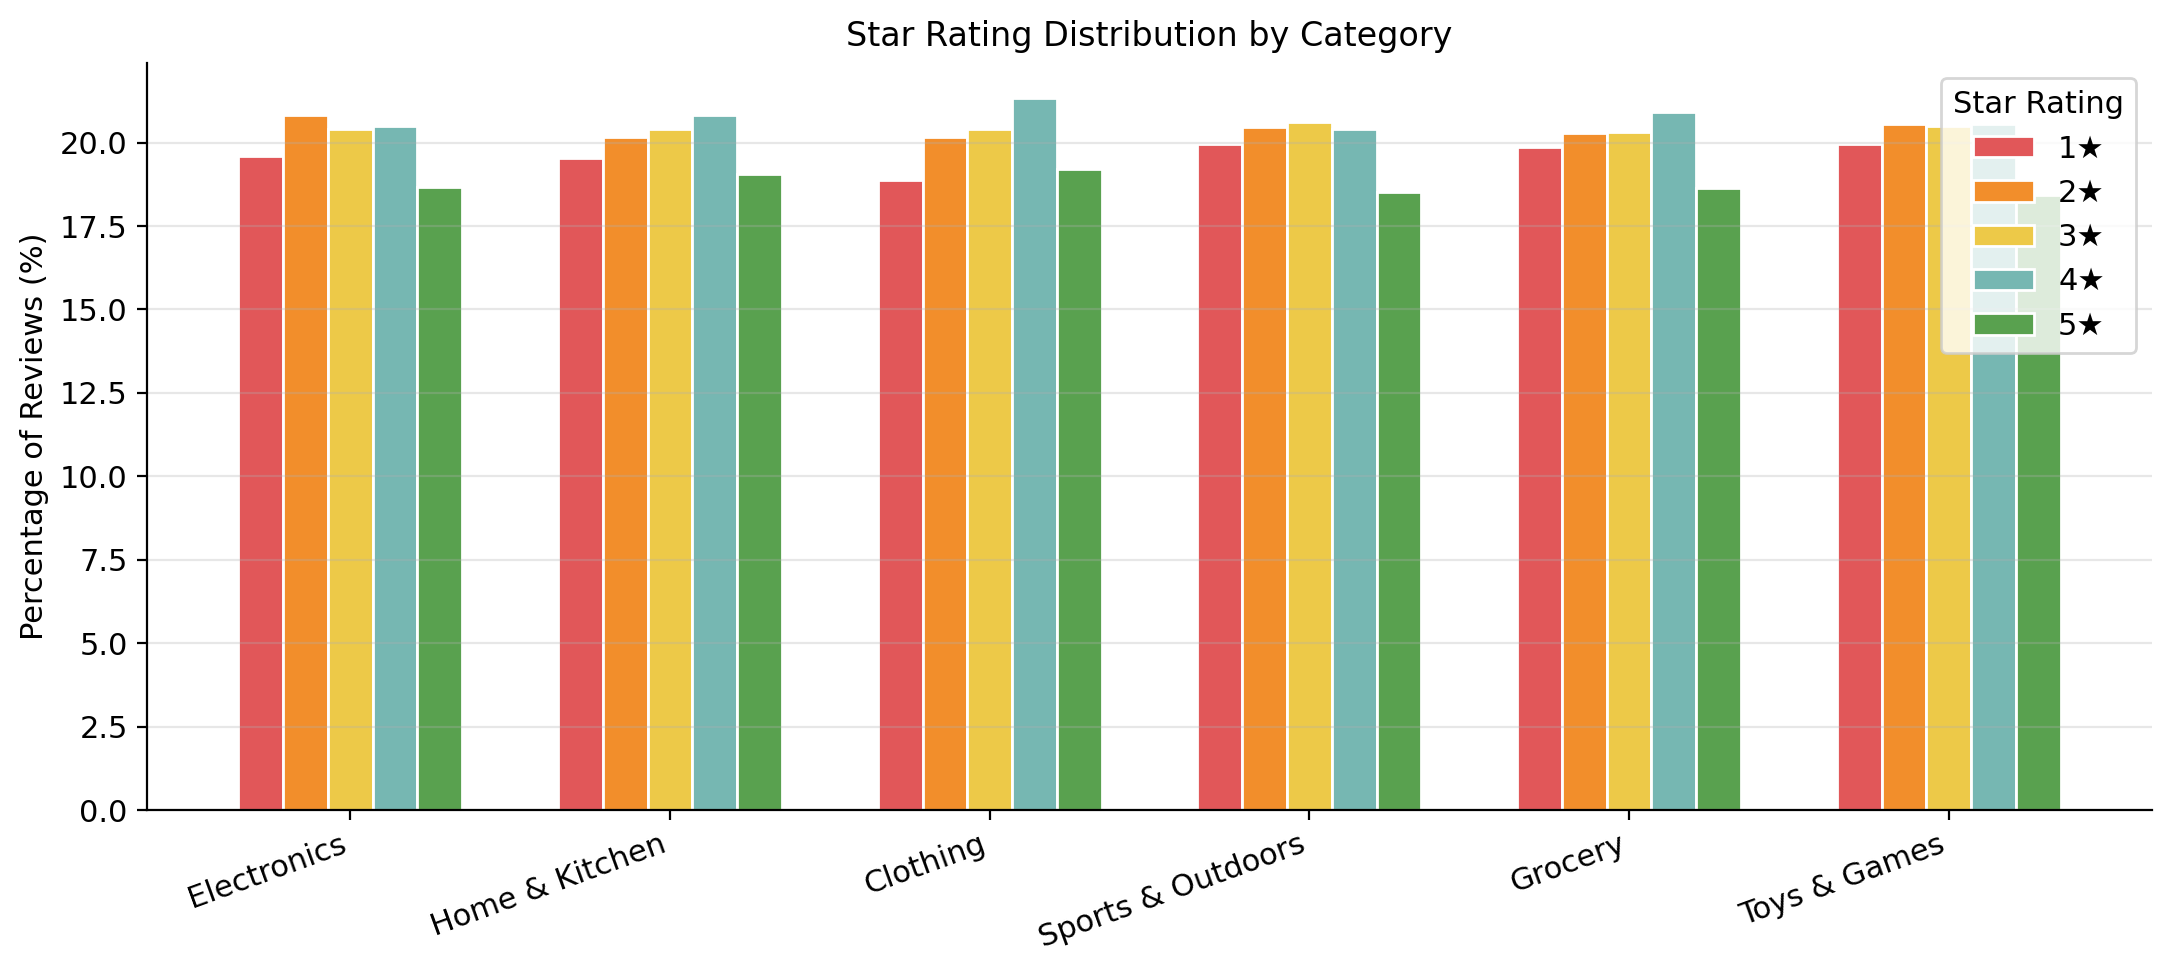
\includegraphics[width=0.9\linewidth]{images/rating_distribution.png}
    \caption{Star rating distribution across six product categories. Each group of five bars represents one star level (1--5).}
    \label{fig:rating_dist}
\end{figure}

\textbf{Evaluation protocol}: Following standard practice for Amazon review sentiment benchmarks \cite{yin2020benchmarking}, 3-star reviews are excluded from binary accuracy computation because their ground-truth sentiment is genuinely ambiguous. All 172,718 reviews go through the full pipeline; the exclusion only affects the accuracy metric.
\end{justify}

\subsection{Preprocessing}
\begin{justify}
All raw review text is cleaned and prepared using SpaCy \cite{spacy2} with the \texttt{en\_core\_web\_sm} model. The steps are:

\begin{enumerate}
    \item \textbf{Cleaning}: HTML entities, URLs, email addresses, and non-ASCII characters are stripped out. Whitespace is normalised.
    \item \textbf{Length filtering}: Reviews under 30 characters or over 2000 characters are dropped — they are typically too short to contain meaningful sentiment or are truncated fragments.
    \item \textbf{Lowercasing and lemmatisation}: Tokens are lowercased and reduced to their base form (e.g., ``running'' $\rightarrow$ ``run'').
    \item \textbf{Stop word removal}: Standard English stop words are removed for the lemmatised text used in topic modelling. The original cleaned text is kept intact for sentiment analysis, since stop words can carry sentiment-relevant information.
    \item \textbf{Implicit negativity detection}: A set of 15 regex patterns flags reviews containing hedging, passive dissatisfaction, or indirect criticism (Table~\ref{tab:implicit_patterns}).
\end{enumerate}

\begin{table}[H]
\centering
\small
\caption{Implicit Negativity Detection Patterns}
\renewcommand{\arraystretch}{1.2}
\begin{tabular}{|l|l|}
\hline
\textbf{Pattern} & \textbf{Example} \\
\hline
\texttt{i\textbackslash s+guess\textbackslash s+it} & ``I guess it works...'' \\
\texttt{not\textbackslash s+(exactly|quite|really)} & ``Not exactly what I expected'' \\
\texttt{would\textbackslash s+not\textbackslash s+recommend} & ``Would not recommend'' \\
\texttt{expected\textbackslash s+(better|more)} & ``Expected better quality'' \\
\texttt{barely\textbackslash s+(works?|functions?)} & ``Barely works after a week'' \\
\texttt{wish\textbackslash s+i\textbackslash s+(had|could|knew)} & ``Wish I had known before'' \\
\texttt{misleading\textbackslash s+description} & ``Misleading description'' \\
\texttt{false\textbackslash s+advertising} & ``False advertising'' \\
\texttt{gave\textbackslash s+it\textbackslash s+a\textbackslash s+chance} & ``Gave it a chance but...'' \\
\texttt{still\textbackslash s+waiting} & ``Still waiting after 3 weeks'' \\
\hline
\end{tabular}
\label{tab:implicit_patterns}
\end{table}
\end{justify}

\subsection{Sentiment Analysis}

\subsubsection{VADER — Lexicon Baseline}
\begin{justify}
VADER \cite{vader} scores each review using its lexicon of 7,517 features. The compound score is computed as:

\begin{equation}
    s_c = \frac{\sum_{i} s_i}{\sqrt{\sum_{i} s_i^2 + \alpha}}, \quad \alpha = 15
\end{equation}

and classified as:
\begin{equation}
    \hat{y}_{\text{VADER}} = \begin{cases} \text{Positive} & s_c \geq 0.05 \\ \text{Negative} & s_c \leq -0.05 \\ \text{Neutral} & \text{otherwise} \end{cases}
\end{equation}

VADER serves as a fast, interpretable baseline and contributes a calibration signal to the fusion step.
\end{justify}

\subsubsection{DistilBERT — Transformer Baseline}
\begin{justify}
DistilBERT \cite{sanh2019distilbert} is a 66M-parameter distillation of BERT, fine-tuned on SST-2 \cite{socher2013recursive}. It outputs binary labels (positive/negative) with a softmax confidence score, tokenising input to at most 512 tokens. This model is included as a paper comparison baseline only; its binary output and SST-2 training distribution make it poorly suited as the primary model for product reviews.
\end{justify}

\subsubsection{RoBERTa — Primary Model}
\begin{justify}
The primary classifier is \texttt{cardiffnlp/twitter-roberta-base-\allowbreak{}sentiment-latest} \cite{barbieri2020tweeteval}, a RoBERTa-base \cite{liu2019roberta} model fine-tuned on 124 million tweets. It outputs a probability distribution over three classes:

\begin{equation}
    P(y \mid x) = \text{softmax}(\mathbf{W} \cdot \text{RoBERTa}(x) + \mathbf{b}), \quad y \in \{\text{negative, neutral, positive}\}
\end{equation}

The predicted label is $\hat{y}_{\text{RoBERTa}} = \arg\max_{y} P(y \mid x)$ with confidence $\hat{p} = \max_{y} P(y \mid x)$.

A signed confidence is derived for the fusion step:
\begin{equation}
    r = \text{sign}(\hat{y}_{\text{RoBERTa}}) \cdot \hat{p}, \quad \text{sign}(\cdot) = \begin{cases} +1 & \text{positive} \\ 0 & \text{neutral} \\ -1 & \text{negative} \end{cases}
\end{equation}
\end{justify}

\subsubsection{Sentiment Fusion}
\begin{justify}
The final sentiment score combines VADER and RoBERTa with a weighted sum:

\begin{equation}
    \boxed{S = 0.4 \cdot s_c^{\text{VADER}} + 0.6 \cdot r^{\text{RoBERTa}}}
    \label{eq:fusion}
\end{equation}

The 60\% weight on RoBERTa reflects its better domain fit; the 40\% on VADER keeps the heuristic signals (punctuation, capitalisation) in play. If the implicit negativity flag is set, a small penalty is applied:

\begin{equation}
    S' = S - 0.05 \cdot \mathbb{1}[\text{implicit\_negative}]
\end{equation}

The score is clipped to $[-1, 1]$ and classified using slightly wider thresholds than VADER alone (reflecting higher transformer confidence):

\begin{equation}
    \hat{y}_{\text{fused}} = \begin{cases} \text{Positive} & S' \geq 0.10 \\ \text{Negative} & S' \leq -0.10 \\ \text{Neutral} & \text{otherwise} \end{cases}
\end{equation}
\end{justify}

\subsection{Topic Modelling}

\subsubsection{Sentence Embeddings}
\begin{justify}
Each lemmatised review is encoded using \texttt{all-MiniLM-L6-v2} \cite{reimers2019sentencebert}, a sentence transformer trained with contrastive learning to produce semantically meaningful 384-dimensional vectors. The embedding of review $d$ is $\mathbf{e}_d \in \mathbb{R}^{384}$.
\end{justify}

\subsubsection{Dimensionality Reduction}
\begin{justify}
Running HDBSCAN directly on 384-dimensional vectors is computationally expensive and degrades clustering quality due to the curse of dimensionality. UMAP \cite{mcinnes2018umap} is used to reduce $\mathbf{e}_d$ down to five dimensions:

\begin{equation}
    p_{j|i} = \exp\!\left(\frac{-\max(0, d(\mathbf{e}_i, \mathbf{e}_j) - \rho_i)}{\sigma_i}\right)
\end{equation}

where $d(\cdot, \cdot)$ is Euclidean distance, $\rho_i$ is the nearest-neighbour distance, and $\sigma_i$ normalises the local density. The low-dimensional embedding minimises cross-entropy between the high- and low-dimensional fuzzy representations. Parameters used: \texttt{n\_neighbors=15}, \texttt{min\_dist=0.0}.
\end{justify}

\subsubsection{Clustering}
\begin{justify}
HDBSCAN \cite{campello2013density} clusters the reduced vectors. It converts the space to a mutual reachability distance:

\begin{equation}
    d_{\text{mreach}}(a, b) = \max\!\left(\text{core}_k(a),\, \text{core}_k(b),\, d(a, b)\right)
\end{equation}

where $\text{core}_k(a)$ is the distance from point $a$ to its $k$-th nearest neighbour. A minimum spanning tree is built over this space and clusters are extracted by varying the density threshold. Points in low-density regions are labelled $-1$ (noise).
\end{justify}

\subsubsection{Topic Representation}
\begin{justify}
For each topic cluster $c$, c-TF-IDF scores identify the most representative terms:

\begin{equation}
    \text{c-TF-IDF}_{t,c} = \frac{f_{t,c}}{W_c} \cdot \log\!\left(1 + \frac{A}{f_t}\right)
\end{equation}

where $f_{t,c}$ is the count of term $t$ in cluster $c$, $W_c = \sum_t f_{t,c}$ is the total word count in the cluster, $A = N / |C|$ is the average words per cluster, and $f_t$ is the total frequency of term $t$ across all documents. The top-4 terms by c-TF-IDF score form the human-readable topic label (e.g., \texttt{battery\_life\_hours\_charge}).
\end{justify}

\subsubsection{Outlier Reduction}
\begin{justify}
After the initial topic assignment, noise reviews (topic $= -1$) are reassigned using cosine similarity to c-TF-IDF cluster centroids:

\begin{equation}
    \hat{z}_d = \arg\max_{c \in C} \cos\!\left(\mathbf{e}_d,\, \boldsymbol{\mu}_c^{\text{c-TF-IDF}}\right)
\end{equation}

where $\boldsymbol{\mu}_c^{\text{c-TF-IDF}}$ is the centroid of cluster $c$ in c-TF-IDF space. This step reduces noise from 31--47\% per category to below 1\% without requiring any re-embedding — a key efficiency advantage.
\end{justify}

\subsubsection{Global Topic Modelling}
\begin{justify}
In addition to the six per-category models, a single global BERTopic model is trained on all 172,718 reviews together. This surfaces cross-category themes — delivery, packaging, customer service — that do not show up clearly when categories are modelled in isolation.
\end{justify}

\subsection{Business Intelligence Extraction}

\subsubsection{Priority Matrix}
\begin{justify}
For each topic $t$ within a category, a priority score quantifies how urgently it needs attention:

\begin{equation}
    \text{Priority}(t) = 0.4 \cdot \frac{N_t}{\max_j N_j} + 0.6 \cdot \frac{|\{d : d \in t,\, \hat{y}_d = \text{Negative}\}|}{N_t}
    \label{eq:priority}
\end{equation}

where $N_t$ is the total number of reviews for topic $t$. The frequency term (weighted 0.4) prevents high-negativity but low-volume niche topics from dominating the priority list — a complaint affecting 200 customers matters less than one affecting 3,000, even if the negativity rate is similar.
\end{justify}

\subsubsection{Category Scorecard}
\begin{justify}
For each category $c$, a summary scorecard is computed:

\begin{equation}
    \bar{S}_c = \frac{1}{N_c} \sum_{d \in c} S_d', \quad \text{NPS-proxy}_c = \frac{|\{d : \hat{y}_d = \text{Positive}\}| - |\{d : \hat{y}_d = \text{Negative}\}|}{N_c}
\end{equation}

The scorecard also includes average star rating, sentiment class breakdown, implicit negativity rate, number of discovered topics, and the top complaint and praise topics.
\end{justify}

\subsubsection{Aspect-Level Sentiment}
\begin{justify}
Eight product aspects are defined with associated keyword sets: Quality, Price/Value, Delivery, Performance, Design/Look, Packaging, Customer Service, and Ease of Use. For each aspect $a$ and category $c$, the mean sentiment is computed over reviews that mention the aspect:

\begin{equation}
    \bar{S}_{a,c} = \frac{1}{|D_{a,c}|} \sum_{d \in D_{a,c}} S_d', \quad D_{a,c} = \{d \in c : \text{keywords}(a) \subset d\}
\end{equation}

The aspect-level negative ratio $\rho_{a,c} = \frac{|\{d \in D_{a,c} : \hat{y}_d = \text{Negative}\}|}{|D_{a,c}|}$ identifies which dimensions are most problematic per category.
\end{justify}

\subsubsection{LLM Agent}
\begin{justify}
A conversational agent powered by LLaMA-3.3-70B via the Groq API receives the structured BI context (priority topics, aspect scores, sample reviews) as a system-level prompt and answers natural language queries about the analysis. The agent supports auto-generated per-category reports and a multi-turn chat interface for ad-hoc questions.
\end{justify}

\subsection{System Architecture and Implementation}
\begin{justify}
The pipeline is implemented in Python 3.14 using the following primary libraries: HuggingFace Transformers \cite{wolf2020transformers} for DistilBERT and RoBERTa inference, BERTopic \cite{grootendorst2022bertopic} for topic modelling, vaderSentiment for VADER, Sentence-Transformers \cite{reimers2019sentencebert} for embeddings, SpaCy \cite{spacy2} for preprocessing, Pandas/NumPy for data manipulation, and Streamlit for the dashboard.

Total pipeline runtime on a MacBook with an Apple M-series chip is approximately 4 hours for all 172,718 reviews, with RoBERTa inference (batch size 64, CPU) accounting for roughly 3.5 hours of that.
\end{justify}
